\section{Additional Experimental Details}

\subsection{Synthetic Experiments}

In this section, we first provide our protocol for generating synthetic data, which is fixed across our synthetic experiments. We then discuss the details of the experiments performed for each of the plots in \autoref{sec:theory} and \autoref{sec:applications}.

\paragraph{Generating synthetic data}

We use the same synthetic data distributions for all of our synthetic experiments. We set the number of sources to $m=10$, and draw accuracies uniformly from $[.55,.75]$, both of which would be typical in relevant applications (ex., in weak supervision). We report these accuracies in \autoref{tab:synthetic_accuracies}. For experiments with dependencies, when $d=1$ we add the edge $(0,1)$, when $d=2$ we add a second edge $(2,3)$ and so on. Every dependency is fixed at $\varepsilon_{ij}=\mathbb{E}[\lambda_i\lambda_j]-\mathbb{E}[\lambda_i]\mathbb{E}[\lambda_j]=0.1$.

\begin{table}[t]
\vskip 0.15in
\renewcommand{\arraystretch}{1.25} % Default value: 1
\begin{center}
\begin{small}
\begin{tabular}{l|cccccccccccr}
\hline
$i$ & 0 & 1 & 2 & 3 & 4 & 5 & 6 & 7 & 8 & 9\\
\hline
Accuracy & .6893 & .6072 & .5954 & .6603 & .6939 & .6346 & .7462 & .6870 & .6462 & .6284 \\
\hline
\end{tabular}
\end{small}
\end{center}
\vskip -0.1in
\caption{The source accuracies used for synthetic experiments. They were each drawn uniformly from $[.55,.75]$.}
\label{tab:synthetic_accuracies}
\end{table}

\paragraph{\autoref{fig:gen_err}: Excess generalization error} 

We measure the expected excess generalization error for several different estimators and values of $n$. For each value of $n$, we take $1000$ samples and measure the generalization error of an estimator trained on this sample. We average the results over these $1000$ samples.

\paragraph{\autoref{fig:data_value_ratio}: Computing the data value ratio}

We compute the data value ratio for unlabeled models with mean and median aggregation for different numbers of dependencies $d$. The definition of the data value ratio requires finding the smallest $n_L$ with which learning from $n_L$ labeled points achieves lower expected generalization error than learning from $n_U$ unlabeled points. To measure the expected generalization error for some $n$, we average over $1000$ samples, which would be intractable to do for every $n_L$. So, we measure the expected generalization error for every $n_L$ between $10$ and $100$, every $n_L$ divisible by $2$ between $100$ and $1000$ and every $n_L$ divisible by $10$ between $1000$ and $5000$. Besides this shortcut, we compute the data value ratio according to its definition.

\paragraph{\autoref{fig:combined}: Combining labeled and unlabeled data}

We compare the practical approach of weighting the unlabeled and labeled estimators according to \cite{GreenStrawderman2001}, formally defined in section \ref{subsec:combined}, with the optimal weight. We let the optimal weight vary with $n_U$ and $n_L$, but not with the specific data points drawn. In other words, we compute the optimal weight to be that which minimizes the average generalization error over $1000$ trials for each $n_L$. On the other hand, the weight from \cite{GreenStrawderman2001} is a function of the learned accuracies (and thus of the specific data points drawn). In \autoref{fig:combined_with_alphas} we report the optimal $\alpha$ for each $n_L$ ($n_U$ is fixed at $1000$) as well as the \textit{average} weight from \cite{GreenStrawderman2001} over $1000$ trials.

\begin{figure}
    \centering
    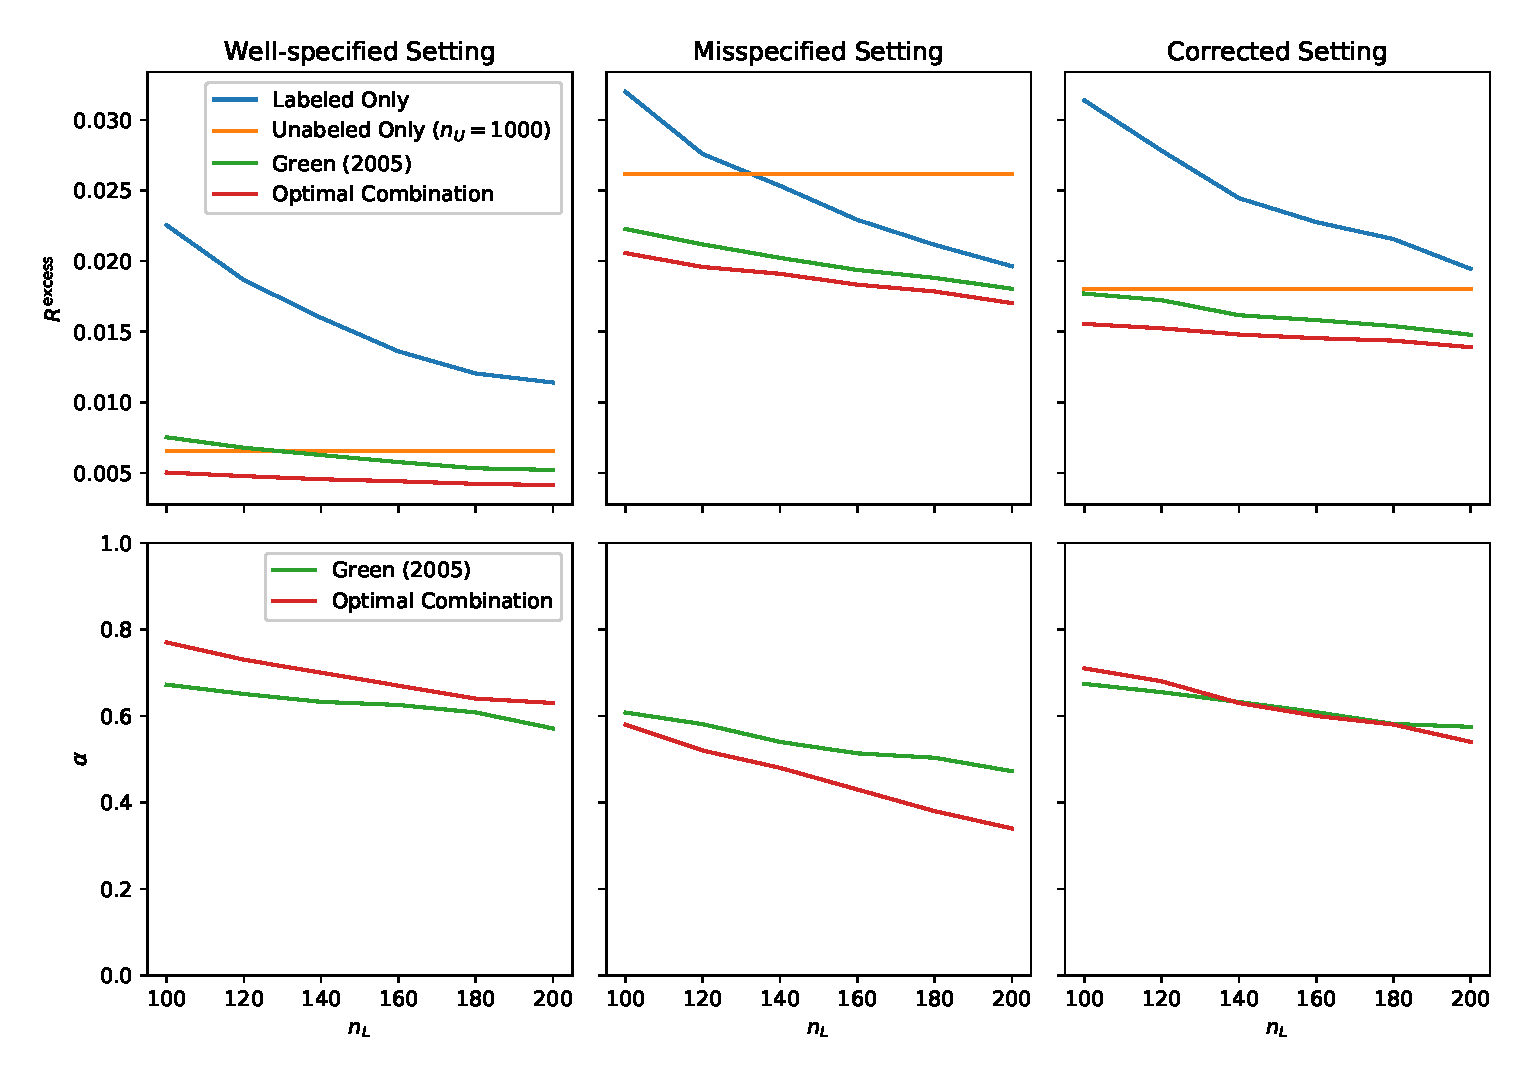
\includegraphics[width=.6\textwidth]{eps_figures/combined_with_alphas.eps}
    %
    \caption{Excess generalization error and associated combination weight $\alpha$ for an optimally weighted combination of labeled and unlabeled estimators, and a combination weighted according to \cite{GreenStrawderman2001} across the well-specified (left), misspecified (center), and corrected (right) settings. The number of unlabeled points is fixed at $n_U=1000$.}
    \label{fig:combined_with_alphas}
\end{figure}

\subsection{Real-World Case Study: Weak Supervision}

We discuss the weak supervision dataset we create and clarify the details of our experimental protocol for the real-world case study.

\paragraph{Creating a weak supervision dataset}

In weak supervision, soft labels from latent variable estimation are used as an alternative to a hand-labeled dataset. The sources used are usually heuristics which incorporate domain-specific knowledge about a particular task and can be acquired relatively cheaply. For our real-world case study, we choose the simple sentiment analysis task of classifying IMDB reviews as positive or negative. Our sources are defined simply: for a collection of positive sentiment words, output ``yes'' if the word appears in the review and ``no'' otherwise; for a collection of negative sentiment words, similarly output ``no'' if the word appears and ``yes'' otherwise. The specific words used and their sentiments are reported in \autoref{tab:imdb_words}. We select these words because they are empirically predictive, appear relatively frequently in reviews and are intuitively associated with positive/negative reviews.

\begin{table}[t]
\vskip 0.15in
\renewcommand{\arraystretch}{1.25} % Default value: 1
\begin{center}
\begin{small}
\begin{tabular}{l|cccccccccccccr}
\hline
Word & love & like & good & great & best & excellent & terrible & worst & bad & better & could & would \\
\hline
Sentiment & + & + & + & + & + & + & - & - & - & - & - & - \\
\hline
\end{tabular}
\end{small}
\end{center}
\vskip -0.1in
\caption{The words used as sources for the real-world weak supervision task of classifying IMDB reviews as positive or negative.}
\label{tab:imdb_words}
\end{table}

\paragraph{\autoref{fig:real_biases_data_value_ratio} and \autoref{tab:real_combo}: Experiments with real data} We measure excess generalization error, the data value ratio and the performances of combined estimators for the real-world dataset. Our protocols for these experiments mirror those we used for synthetic datasets, with two key differences: (1) for each trial, we sample points uniformly from the training set of 40,000 points, since we cannot sample directly from the distribution and (2) we measure generalization error on the test set, since we cannot compute the expected generalization error directly.